\documentclass[onlytextwidth]{beamer}
\documentclass[onlytextwidth]{beamer}
\usepackage[utf8]{inputenc}
\usepackage{microtype}
\usepackage{amsmath}
\usepackage{amssymb}
\usepackage[nomessages]{fp} %\FPeval{\var-name}{2*sin(pi/6)}
\usepackage{siunitx} %units in math. eg 20\milli\meter
\usepackage{yhmath} % for arcs, overparenth command
\usepackage{tikz} %graphics
\usetikzlibrary{quotes, angles}
%\usepackage{graphicx} already loaded by beamer class
%consider setting \graphicspath{{images/}}
%\parskip ?? to avoid paragraph indent
\usepackage{multicol} %may not need this package, just columns environment
\usepackage{venndiagram}

\subtitle[BECA]{Bronx Early College Academy}
\author[Huson]{Christopher J. Huson PhD}

\setbeamertemplate{headline}{\vskip2mm 
  BECA / \insertshortauthor \, / \inserttitle
  \hfill 
  \insertsection
  }

\title{Geometry Unit 8: Congruence transformations}
\date{1 January - 13 January 2023}

\begin{document}
\frame{\titlepage}

\section[Outline]{}
\frame{\tableofcontents}


\section{8.1 Translation, equilateral triangle construction \hfill 1 January}
\begin{frame}{Learning Target: I can translate objects}
{CCSS: HSG.CO.C.9 Prove geometric theorems \hfill \alert{4.1}}
  \begin{block}{Four pages of $\triangle$ duplication constructions for binder}
    \begin{enumerate}
        \item Side-side-side (SSS)
        \item Side-angle-side (SAS)
        \item Angle-side-angle (ASA)
        \item Side-side-angle (SSA), false, ``ambiguous case"
    \end{enumerate}
  \end{block}
\end{frame}

\begin{frame}{SAS triangle congruence}
  \begin{block}{SAS $\triangle$ congruence}
    \begin{enumerate}
        \item SAS $\triangle$ congruence Angle must be the \emph{included} angle, between the two sides
        \item Duplicate a side, duplicate an angle, duplicate a side.
        \item $\triangle ABC \cong \triangle A'B'C'$ iff $\overline{AB} \cong \overline{A'B'}, \angle A \cong \angle A', \text{ and } \overline{AC} \cong \overline{A'C'}$
        \item Angle-side-angle (ASA) $\triangle ABC \cong \triangle A'B'C'$ iff $\angle A \cong \angle A', \overline{AB} \cong \overline{A'B'}, \text{ and } \angle B \cong \angle B'$
        \item Duplicate an angle, duplicate a side, duplicate an angle
         \item SSA $\triangle$ congruence (or ASS, ``jack ass theorem")
        \item Duplicate an angle, duplicate a side, duplicate an side
        \item Given $\triangle ABC$ if $ \angle A \cong \angle A', \overline{AB} \cong \overline{A'B'}, \text{ and } \overline{BC} \cong \overline{B'C'}$ then two possible $\triangle$s may result.
         \item  ff
      \end{enumerate}
    \end{block}
\end{frame}

\section{8.5 Translation, equilateral triangle construction \hfill 10 January}
\begin{frame}{When does a transformations maintain length and angle measures?}
  Triangle $A'B'C'$ is the image of triangle $ABC$ after a translation of 2 units to the right and 3 units up. Is triangle $ABC$ congruent to triangle $A'B'C'$ ? Explain why.\\[0.25cm]
  \pause \includegraphics[width=0.9\textwidth]{../graphics/isometry_JN2018-25-sol.png}\\
  \pause \includegraphics[width=0.9\textwidth]{../graphics/isometry_JN2018-25-sol2.png}
\end{frame}

\begin{frame}{Symmetry}
  {When is an object unchanged by a transformation?}
  If when an object $A \rightarrow A'$ and $A = A'$ then we say it is symmetric. \\
  Reflection: \emph{axis of symmetry}\\
  Rotation: \emph{center and angle of rotation}\\[0.25cm]
  Example: Regular polygons are symmetrical\\[0.25cm]
  \pause 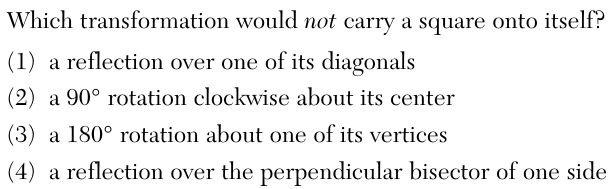
\includegraphics[width=0.7\textwidth]{../graphics/symmetry-square_JA2018-15.png}\\
  \pause 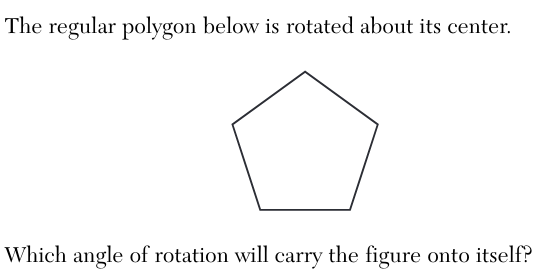
\includegraphics[width=0.7\textwidth]{../graphics/symmetry_JN2018-19.png}
\end{frame}





\section{8.4 Translation, equilateral triangle construction \hfill 6 January}
\begin{frame}{Learning Target: I can translate objects}
{CCSS: HSG.CO.C.9 Prove geometric theorems \hfill \alert{8.1}}
  \begin{block}{Four pages of $\triangle$ duplication for your binder}
    \begin{enumerate}
        \item Side-side-side (SSS $\triangle \cong$)\\
        $\triangle ABC \cong \triangle A'B'C'$ iff $\overline{AB} \cong \overline{A'B'}, \overline{BC} \cong \overline{B'C'}, \text{ and } \overline{AC} \cong \overline{A'C'}$
        \item Side-angle-side (SAS)
        \item Angle-side-angle (ASA)
        \item Side-side-angle (SSA), false, ``ambiguous case"
    \end{enumerate}
    \end{block}
    Function notation: $A \rightarrow A'$ is pronounced ``A gets mapped to A prime," or ``A corresponds to A prime."
  \end{frame}

\section{SSS Triangle congruence \hfill 1 January}
\begin{frame}{SSS Triangle congruence (``side-side-side")}
  Given $\triangle ABC$, duplicate $\triangle ABC$ by duplicating each side.
    \begin{enumerate}
      \item Construct $\overrightarrow{A'}$.
      \item Circle $A'$ with radius $AB$. Intersection $B'$.
      \item Circle $A'$ with radius $AC$.
      \item Circle $B'$ with radius $BC$. Intersection $C'$.
      \item $\triangle ABC \cong \triangle A'B'C'$ by the SSS $\triangle \cong$ Postulate.
    \end{enumerate}
    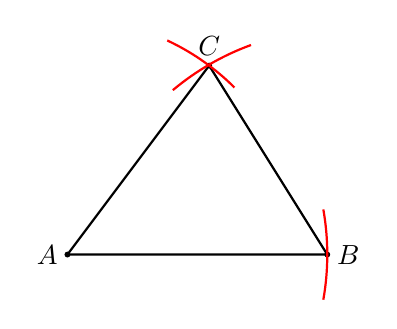
\begin{tikzpicture}[scale=0.6]
      \draw [thick] (0,0)--(5.5,0)--(3,4)--cycle;
      \draw [fill] (0,0) circle [radius=0.05] node[left]{$A$};
      \draw [fill] (5.5,0) circle [radius=0.05] node[right]{$B$};
      \draw [fill] (3,4) circle [radius=0.05] node[above]{$C$};
      \draw[thick,red] ([shift=(-10:5.5)]0,0) arc (-10:10:5.5);
      \draw[thick,red] ([shift=(45:5)]0,0) arc (45:65:5);
      \draw[thick,red] ([shift=(110:4.72)]5.5,0) arc (110:130:5.5);
    \end{tikzpicture}
    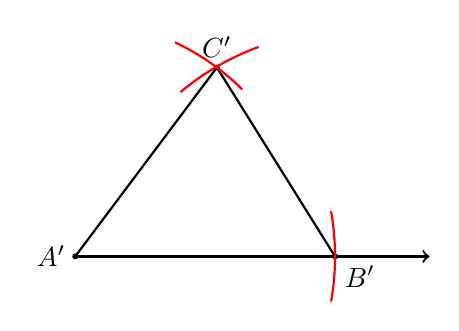
\begin{tikzpicture}[scale=0.6]
      \draw [thick] (0,0)--(5.5,0)--(3,4)--cycle;
      \draw [->, thick] (0,0)--(7.5,0);
      \draw [fill] (0,0) circle [radius=0.05] node[left]{$A'$};
      \draw [fill] (5.5,0) circle [radius=0.05] node[below right]{$B'$};
      \draw [fill] (3,4) circle [radius=0.05] node[above]{$C'$};
      \draw[thick,red] ([shift=(-10:5.5)]0,0) arc (-10:10:5.5);
      \draw[thick,red] ([shift=(45:5)]0,0) arc (45:65:5);
      \draw[thick,red] ([shift=(110:4.72)]5.5,0) arc (110:130:5.5);
    \end{tikzpicture}
  \end{frame}

\section{SAS Triangle congruence \hfill 1 January}
\begin{frame}{SAS Triangle congruence (``side-angle-side")}
  \begin{enumerate}
    \item Given $\triangle ABC$, construct a duplicate $\triangle A'B'C'$
    \item Duplicate side $\overline{AB}$, duplicate $\angle A$, duplicate side $\overline{AC}$
    \item Angle must be the \emph{included} angle, between the two sides
    \item $\triangle ABC \cong \triangle A'B'C'$ iff $\overline{AB} \cong \overline{A'B'}, \angle A \cong \angle A', \text{ \& } \overline{AC} \cong \overline{A'C'}$
  \end{enumerate}
  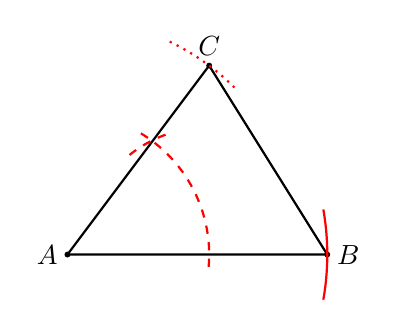
\begin{tikzpicture}[scale=0.6]
    \draw [thick] (0,0)--(5.5,0)--(3,4)--cycle;
    \draw [fill] (0,0) circle [radius=0.05] node[left]{$A$};
    \draw [fill] (5.5,0) circle [radius=0.05] node[right]{$B$};
    \draw [fill] (3,4) circle [radius=0.05] node[above]{$C$};
    \draw[thick, red] ([shift=(-10:5.5)]0,0) arc (-10:10:5.5);
    \draw[thick, dashed,red] ([shift=(-5:3)]0,0) arc (-5:60:3);
    \draw[thick, dashed,red] ([shift=(110:2.7)]3,0) arc (110:130:2.7);
    \draw[thick, dotted,red] ([shift=(45:5)]0,0) arc (45:65:5);
  \end{tikzpicture}
  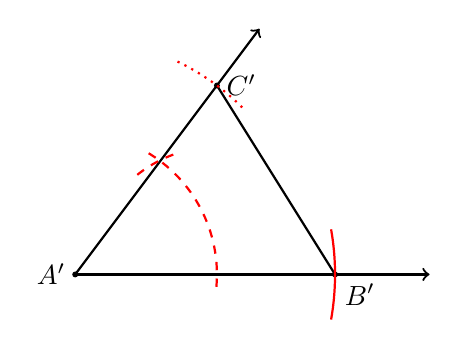
\begin{tikzpicture}[scale=0.6]
    \draw [thick] (5.5,0)--(3,4);
    \draw [->, thick] (0,0)--(7.5,0);
    \draw [->, thick] (0,0)--(3,4)--(3.9,5.2);
    \draw [fill] (0,0) circle [radius=0.05] node[left]{$A'$};
    \draw [fill] (5.5,0) circle [radius=0.05] node[below right]{$B'$};
    \draw [fill] (3,4) circle [radius=0.05] node[right]{$C'$};
    \draw[thick, red] ([shift=(-10:5.5)]0,0) arc (-10:10:5.5);
    \draw[thick, dashed,red] ([shift=(-5:3)]0,0) arc (-5:60:3);
    \draw[thick, dashed,red] ([shift=(110:2.7)]3,0) arc (110:130:2.7);
    \draw[thick, dotted,red] ([shift=(45:5)]0,0) arc (45:65:5);
  \end{tikzpicture}
  \end{frame}

\section{ASA Triangle congruence \hfill 1 January}
\begin{frame}{ASA Triangle congruence (``angle-side-angle")}
  \begin{enumerate}
    \item Given $\triangle ABC$, construct a duplicate $\triangle A'B'C'$
    \item Duplicate $\angle A$, duplicate side $\overline{AB}$, duplicate $\angle B$
    \item One side and \emph{any} two angles ("AAS" is ok)
    \item $\triangle ABC \cong \triangle A'B'C'$ iff $\angle A \cong \angle A', \overline{AB} \cong \overline{A'B'}, \text{ \& } \angle B \cong \angle B'$
  \end{enumerate}
  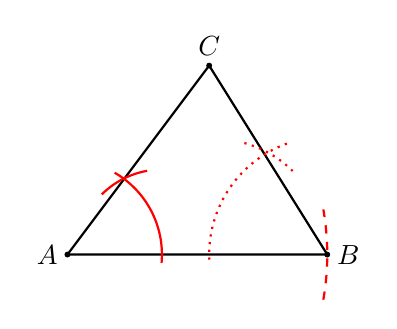
\begin{tikzpicture}[scale=0.6]
    \draw [thick] (0,0)--(5.5,0)--(3,4)--cycle;
    \draw [fill] (0,0) circle [radius=0.05] node[left]{$A$};
    \draw [fill] (5.5,0) circle [radius=0.05] node[right]{$B$};
    \draw [fill] (3,4) circle [radius=0.05] node[above]{$C$};
    \draw[thick, dashed,red] ([shift=(-10:5.5)]0,0) arc (-10:10:5.5);
    \draw[thick, red] ([shift=(-5:2)]0,0) arc (-5:60:2);
    \draw[thick, red] ([shift=(100:1.8)]2,0) arc (100:135:1.8);
    \draw[thick, dotted, red] ([shift=(110:2.5)]5.5,0) arc (110:185:2.5);
    \draw[thick, dotted, red] ([shift=(45:2.5)]3,0) arc (45:75:2.3);
  \end{tikzpicture}
  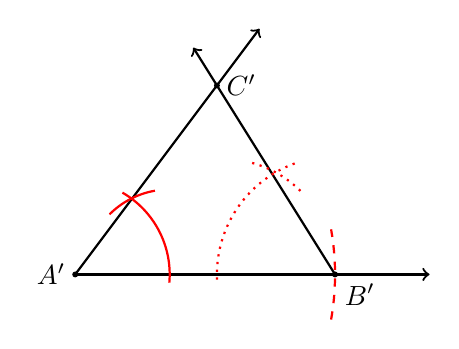
\begin{tikzpicture}[scale=0.6]
    \draw [->, thick] (5.5,0)--(3,4)--(2.5,4.8);
    \draw [->, thick] (0,0)--(7.5,0);
    \draw [->, thick] (0,0)--(3,4)--(3.9,5.2);
    \draw [fill] (0,0) circle [radius=0.05] node[left]{$A'$};
    \draw [fill] (5.5,0) circle [radius=0.05] node[below right]{$B'$};
    \draw [fill] (3,4) circle [radius=0.05] node[right]{$C'$};
    \draw[thick, dashed,red] ([shift=(-10:5.5)]0,0) arc (-10:10:5.5);
    \draw[thick, red] ([shift=(-5:2)]0,0) arc (-5:60:2);
    \draw[thick, red] ([shift=(100:1.8)]2,0) arc (100:135:1.8);
    \draw[thick, dotted, red] ([shift=(110:2.5)]5.5,0) arc (110:185:2.5);
    \draw[thick, dotted, red] ([shift=(45:2.5)]3,0) arc (45:75:2.3);
  \end{tikzpicture}
  \end{frame}

\section{SSA Triangle congruence \hfill 1 January}
\begin{frame}{SSA \emph{false} congruence (ASS or ``jack ass theorem")}
  \begin{enumerate}
    \item Given $\triangle ABC$, two $\triangle$s may have two pairs of congruent sides and a \emph{non-included} congruent angle.
    \item This is called the ``ambiguous case"
    %\item $\triangle ABC \cong \triangle A'B'C'$ iff $\overline{AB} \cong \overline{A'B'}, \angle A \cong \angle A', \text{ \& } \overline{AC} \cong \overline{A'C'}$
  \end{enumerate}
  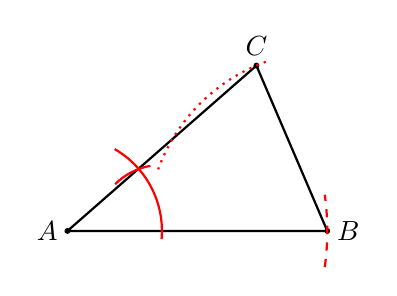
\begin{tikzpicture}[scale=0.6]
    \draw [thick] (0,0)--(5.5,0)--(4,3.5)--cycle;
    \draw [fill] (0,0) circle [radius=0.05] node[left]{$A$};
    \draw [fill] (5.5,0) circle [radius=0.05] node[right]{$B$};
    \draw [fill] (4,3.5) circle [radius=0.05] node[above]{$C$};
    \draw[thick, dashed, red] ([shift=(-8:5.5)]0,0) arc (-8:8:5.5);
    %\draw[thick, red] ([shift=(0:0.75)]0,0) arc (0:37:0.75);
    \draw[thick, red] ([shift=(-5:2)]0,0) arc (-5:60:2);
    \draw[thick, red] ([shift=(100:1.4)]2,0) arc (100:135:1.4);
    \draw[thick, dotted, red] ([shift=(110:3.81)]5.5,0) arc (110:160:3.81);
  \end{tikzpicture}
  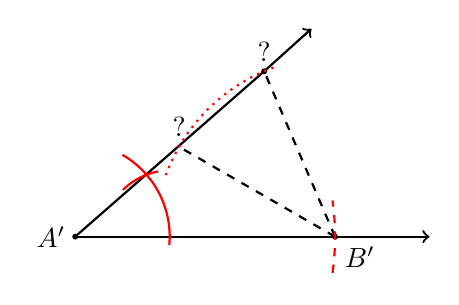
\begin{tikzpicture}[scale=0.6]
    \draw [dashed, thick] (5.5,0)--(4,3.5);
    \draw [dashed, thick] (5.5,0)--(2.2,1.9)node[above]{?};
    \draw [->, thick] (0,0)--(7.5,0);
    \draw [->, thick] (0,0)--(4,3.5)--(5,4.4);
    \draw [fill] (0,0) circle [radius=0.05] node[left]{$A'$};
    \draw [fill] (5.5,0) circle [radius=0.05] node[below right]{$B'$};
    \draw [fill] (4,3.5) circle [radius=0.05] node[above]{?};
    \draw[thick, dashed, red] ([shift=(-8:5.5)]0,0) arc (-8:8:5.5);
    %\draw[thick, red] ([shift=(0:0.75)]0,0) arc (0:37:0.75);
    \draw[thick, red] ([shift=(-5:2)]0,0) arc (-5:60:2);
    \draw[thick, red] ([shift=(100:1.4)]2,0) arc (100:135:1.4);
    \draw[thick, dotted, red] ([shift=(110:3.81)]5.5,0) arc (110:160:3.81);
  \end{tikzpicture}
\end{frame}

\section{HL Triangle congruence \hfill 1 January}
\begin{frame}{HL Triangle congruence (``hypotenuse-leg")}
  Given right $\triangle ABC$, duplicate $\triangle ABC$ by duplicating a leg, the right angle, and the hypotenuse.
  \begin{enumerate}
    \item Construct $\overrightarrow{A'}$.
    \item Circle $A'$ with radius $AB$. Intersection $B'$.
    \item Construct a perpendicular to $\overline{A'B'}$ through $B'$.
    \item Circle $A'$ with radius $AC$. Intersection $C'$.
    \item $\triangle ABC \cong \triangle A'B'C'$ by the HL $\triangle \cong$ theorem.
  \end{enumerate}
  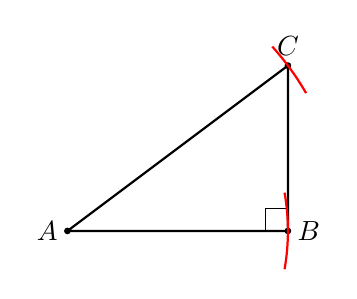
\begin{tikzpicture}[scale=0.7]
    \draw [thick] (0,0)--(4,0)--(4,3)--cycle;
    \draw [fill] (0,0) circle [radius=0.05] node[left]{$A$};
    \draw [fill] (4,0) circle [radius=0.05] node[right]{$B$};
    \draw (4,0) ++(-0.4,0)-- +(0,0.4)-- +(0.4,0.4);
    \draw [fill] (4,3) circle [radius=0.05] node[above]{$C$};
    \draw[thick,red] ([shift=(-10:4)]0,0) arc (-10:10:4);
    \draw[thick,red] ([shift=(30:5)]0,0) arc (30:42:5);
    %\draw[thick,red] ([shift=(110:4.72)]5.5,0) arc (110:130:5.5);
  \end{tikzpicture}
  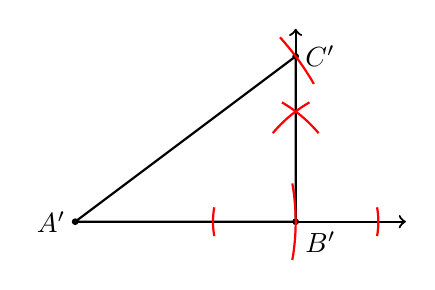
\begin{tikzpicture}[scale=0.7]
    \draw [thick] (0,0)--(4,0)--(4,3)--cycle;
    \draw [->, thick] (0,0)--(6,0);
    \draw [->, thick] (4,0)--(4,3.5);
    \draw [fill] (0,0) circle [radius=0.05] node[left]{$A'$};
    \draw [fill] (4,0) circle [radius=0.05] node[below right]{$B'$};
    \draw [fill] (4,3) circle [radius=0.05] node[right]{$C'$};
    \draw[thick,red] ([shift=(-10:4)]0,0) arc (-10:10:4);
    \draw[thick,red] ([shift=(30:5)]0,0) arc (30:42:5);
    %\draw[thick,red] ([shift=(110:4.72)]5.5,0) arc (110:130:5.5);
    \draw[thick,red] ([shift=(-10:1.5)]4,0) arc (-10:10:1.5);
    \draw[thick,red] ([shift=(170:1.5)]4,0) arc (170:190:1.5);
    \draw[thick,red] ([shift=(40:2.5)]2.5,0) arc (40:60:2.5);
    \draw[thick,red] ([shift=(120:2.5)]5.5,0) arc (120:140:2.5);
  \end{tikzpicture}
\end{frame}


\end{document}